\section{Исследование параметров спейсеров}
Спейсер предназначен для отделения высоколегированной области вырожденного полупроводника от активной. Диффундируя донорная примесь изменяла бы зонную структуру активной (квантовой) области. Так же спейсер препятствует накоплению заряда вблизи барьеров, что влияет на пиковое напряжение и ток.
\subsection{Исследование влияния размеров спейсера}
Рассмотрим спейсеры <<a>>: 
\begin{itemize}
	\item 3 монослоя;
	\item 7 монослоя;
	\item 10 монослоя;
	\item 15 монослоя.
\end{itemize}
\subsubsection{Прозрачность РТГС}

\begin{figure}[h]
	\centering
	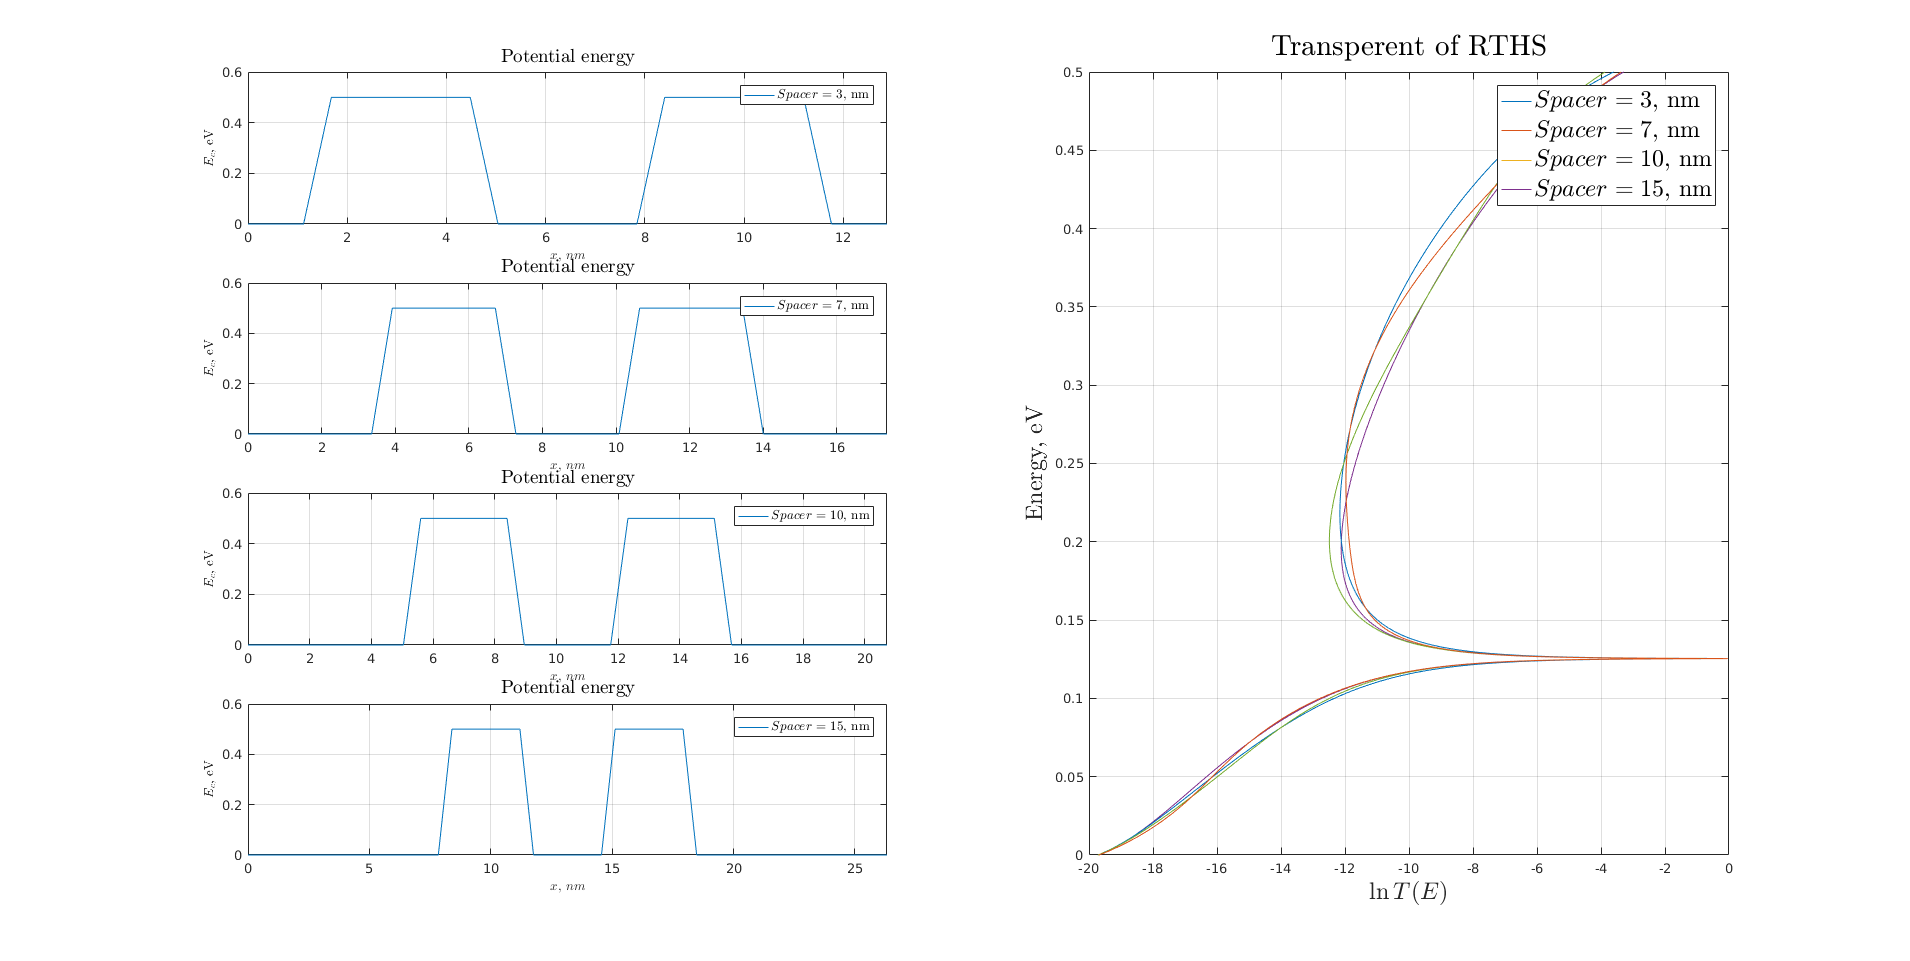
\includegraphics[width=\linewidth]{qslt.png}
	\caption{Прозрачность РТГС при различной ширине спейсеров}
	\label{fig:qslt}
\end{figure}

Прозрачность гетероструктуры изменяется незначительно.

\subsubsection{ВАХ РТГС}
Увеличение размеров спейсера ведет к незначительному (порядок не изменяется), а пиковое напряжение не смещается.

\begin{figure}[h!]
	\centering
	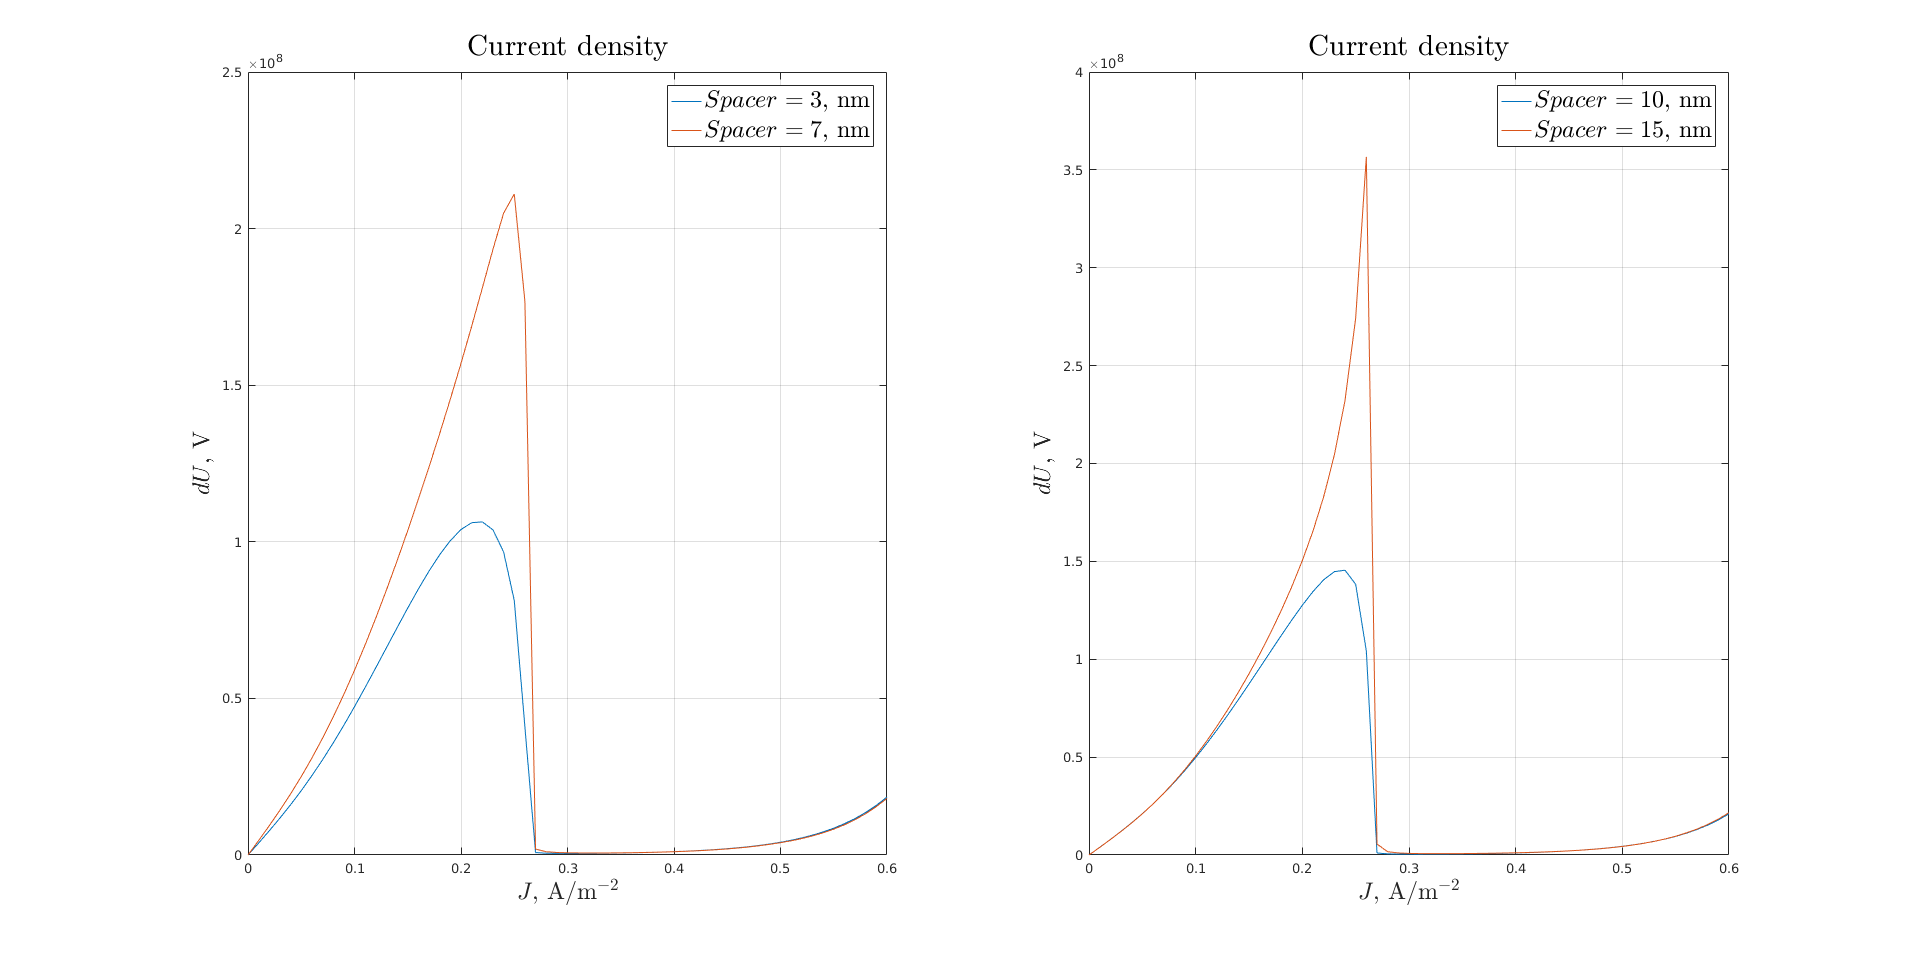
\includegraphics[width=0.9\linewidth]{qslj.png}
	\caption{ВАХ РТГС при различной ширине спейсеров}
	\label{fig:qslj}
\end{figure}


\subsubsection{Учет перераспределения зарядов}
Величина спейсера влияет на накопление заряда вблизи барьеров. Данный эффект сдвигает пиковое напряжение и увеличивает его.

\begin{figure}[h!]
	\centering
	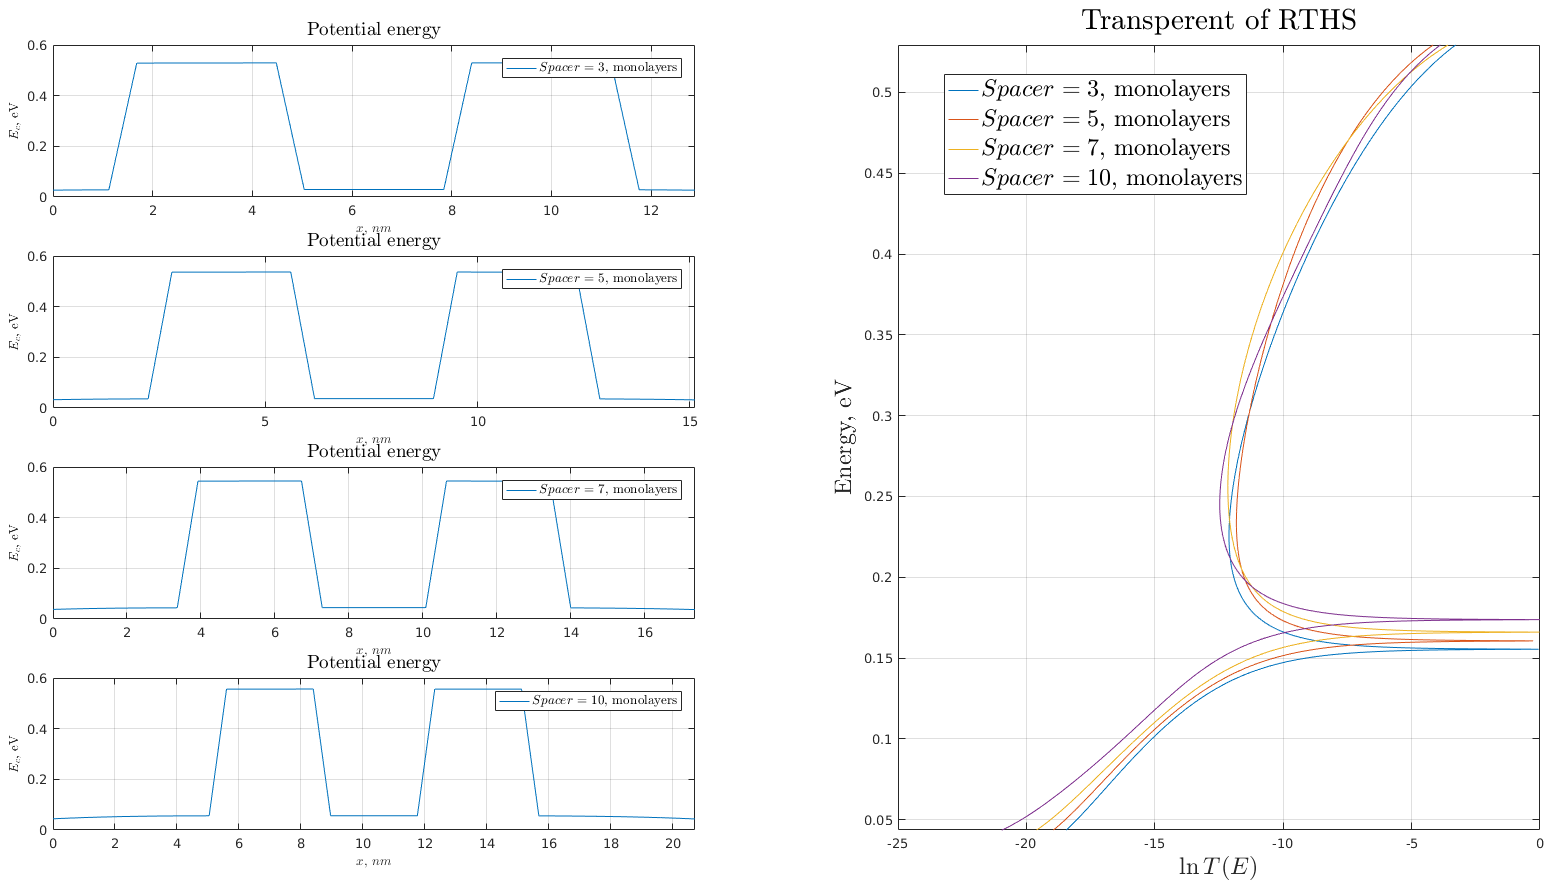
\includegraphics[width=0.9\linewidth]{qslqt.png}
	\caption{Прозрачность РТГС при различной ширине спейсеров с учетом перераспределения заряда}
	\label{fig:qslqt}
\end{figure}

\begin{figure}[h!]
	\centering
	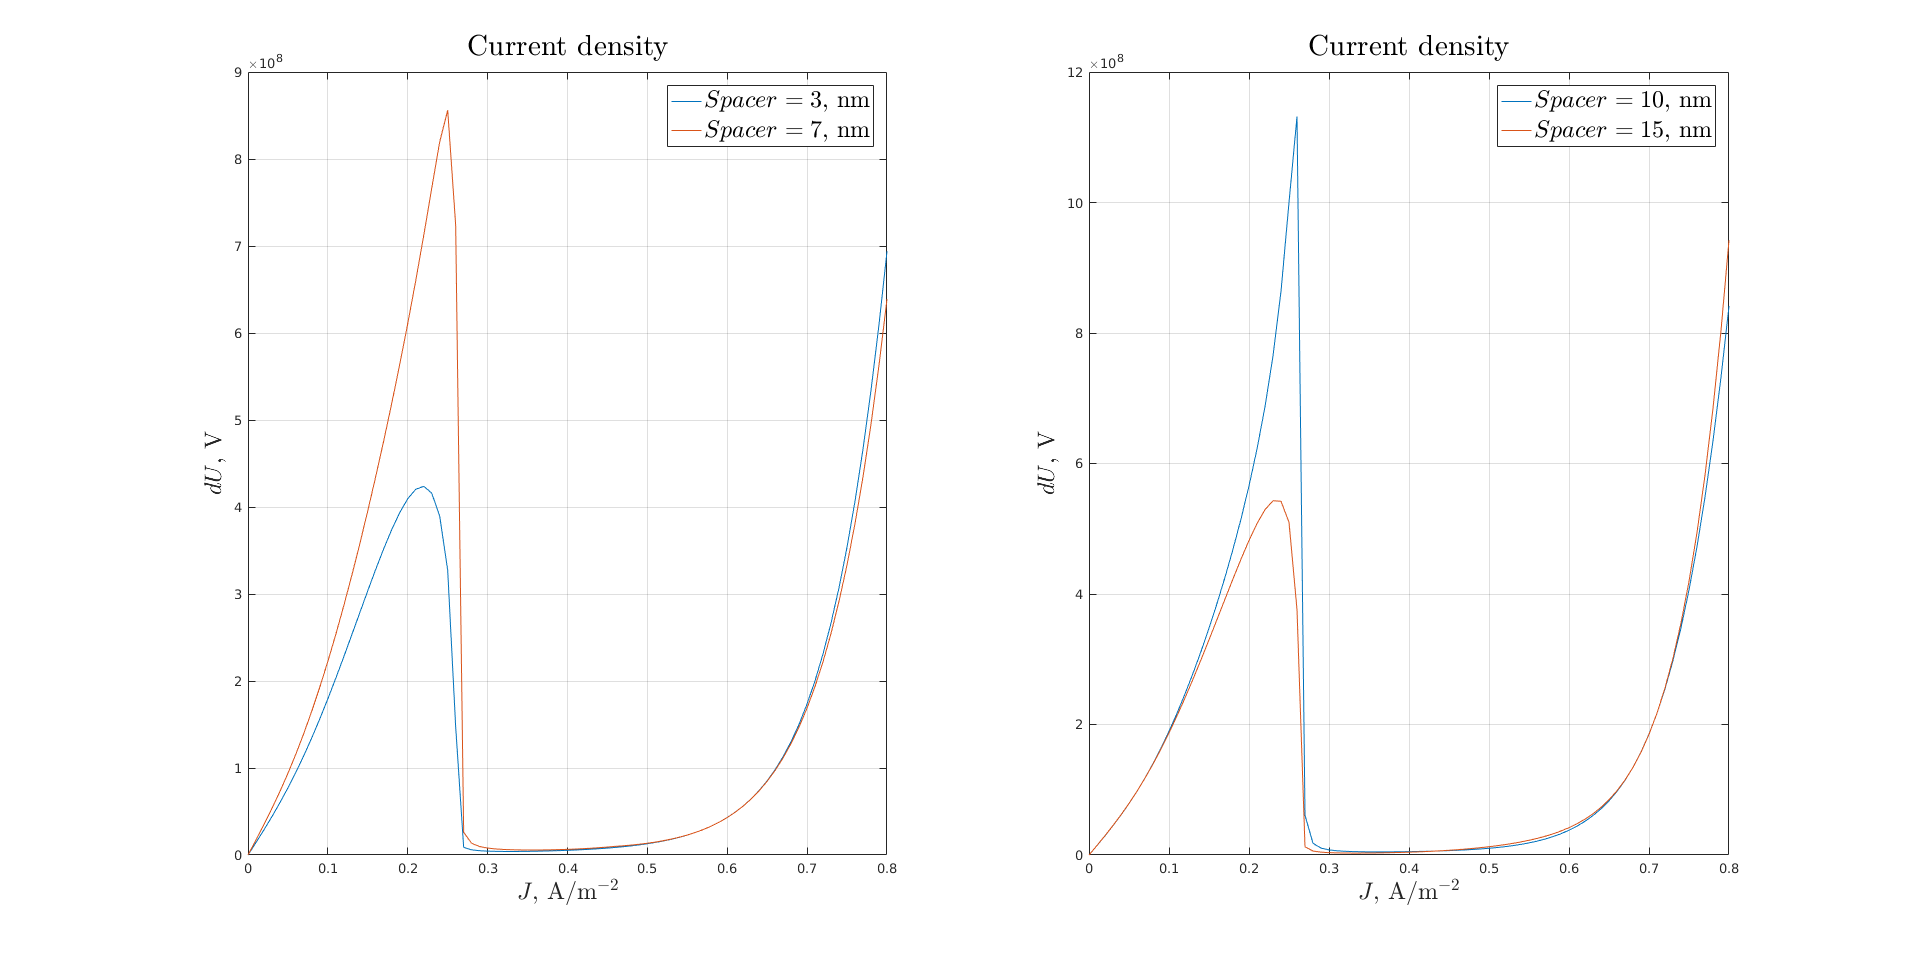
\includegraphics[width=0.9\linewidth]{qslqj.png}
	\caption{ВАХ РТГС при различной ширине спейсеров с учетом перераспределения заряда}
	\label{fig:qslqj}
\end{figure}

\subsection{Вывод}
Из полученных зависимостей видно, что размеры спейсера с учетом перераспределения заряда влияют на ВАХ РТГС при размера менее, чем несколько монослоев. При больших размерах ток через РТГС уменьшается незначительно, так же, как и пиковое напряжение.